\documentclass{sigchi}


%% EXAMPLE BEGIN -- HOW TO OVERRIDE THE DEFAULT COPYRIGHT STRIP -- (July 22, 2013 - Paul Baumann)
% \toappear{Permission to make digital or hard copies of all or part of this work for personal or classroom use is      granted without fee provided that copies are not made or distributed for profit or commercial advantage and that copies bear this notice and the full citation on the first page. Copyrights for components of this work owned by others than ACM must be honored. Abstracting with credit is permitted. To copy otherwise, or republish, to post on servers or to redistribute to lists, requires prior specific permission and/or a fee. Request permissions from permissions@acm.org. \\
% {\emph{CHI'14}}, April 26--May 1, 2014, Toronto, Canada. \\
% Copyright \copyright~2014 ACM ISBN/14/04...\$15.00. \\
% DOI string from ACM form confirmation}
%% EXAMPLE END -- HOW TO OVERRIDE THE DEFAULT COPYRIGHT STRIP -- (July 22, 2013 - Paul Baumann)


% Arabic page numbers for submission.  Remove this line to eliminate
% page numbers for the camera ready copy 

\pagenumbering{arabic}

% Load basic packages
\usepackage{balance}  % to better equalize the last page
\usepackage{graphics} % for EPS, load graphicx instead 
%\usepackage[T1]{fontenc}
\usepackage{txfonts}
\usepackage{times}    % comment if you want LaTeX's default font
\usepackage[pdftex]{hyperref}
% \usepackage{url}      % llt: nicely formatted URLs
\usepackage{color}
\usepackage{textcomp}
\usepackage{booktabs}
\usepackage{ccicons}
\usepackage{todonotes}

% llt: Define a global style for URLs, rather that the default one
\makeatletter
\def\url@leostyle{%
  \@ifundefined{selectfont}{\def\UrlFont{\sf}}{\def\UrlFont{\small\bf\ttfamily}}}
\makeatother
\urlstyle{leo}

% To make various LaTeX processors do the right thing with page size.
\def\pprw{8.5in}
\def\pprh{11in}
\special{papersize=\pprw,\pprh}
\setlength{\paperwidth}{\pprw}
\setlength{\paperheight}{\pprh}
\setlength{\pdfpagewidth}{\pprw}
\setlength{\pdfpageheight}{\pprh}

% Make sure hyperref comes last of your loaded packages, to give it a
% fighting chance of not being over-written, since its job is to
% redefine many LaTeX commands.
\definecolor{linkColor}{RGB}{6,125,233}
\hypersetup{%
  pdftitle={SIGCHI Conference Proceedings Format},
  pdfauthor={LaTeX},
  pdfkeywords={SIGCHI, proceedings, archival format},
  bookmarksnumbered,
  pdfstartview={FitH},
  colorlinks,
  citecolor=black,
  filecolor=black,
  linkcolor=black,
  urlcolor=linkColor,
  breaklinks=true,
}

% create a shortcut to typeset table headings
% \newcommand\tabhead[1]{\small\textbf{#1}}

% End of preamble. Here it comes the document.
  \begin{document}

\title{Quantitative Evaluation of Touch-Screen Performance with
  Transition Matrix Measures}

\numberofauthors{3}
\author{%
  \alignauthor{1st Author Name\\
    \affaddr{Affiliation}\\
    \affaddr{City, Country}\\
    \email{e-mail address}}\\
  \alignauthor{2nd Author Name\\
    \affaddr{Affiliation}\\
    \affaddr{City, Country}\\
    \email{e-mail address}}\\
  \alignauthor{3rd Author Name\\
    \affaddr{Affiliation}\\
    \affaddr{City, Country}\\
    \email{e-mail address}}\\
}

\maketitle

\begin{abstract}
  HCI systems for supporting collaborative creativity are often
  evaluated with user ratings and interviews. However, such data can
  be impractical to collect in-the-wild, such as during musical
  performances. In this paper we consider measures of gestural
  transitions during collaborative interactions with musical touch
  screen interfaces. The performers' interactions are characterised as
  sequences of discrete gestures and summarised in a transition matrix
  for each performance. Using a corpus of more than 140 performances,
  rehearsals, and demonstrations, we find that two matrix measures,
  flux and entropy, vary significantly with different kinds of
  in-the-wild interactions. Further, using performers' ratings
  collected during a lab-study we find that these measures have a
  significant relationship with the perceived effect of the interface
  on performance. Thus transition analysis, flux and entropy, can be
  used as a proxy for performer ratings during in-the-wild interaction.
\end{abstract}

\keywords{  Creativity Support Tools;
  Agent; 
  Design;
  Methodology}

\category{H.5.5.}{Information Interfaces and Presentation
  (e.g. HCI)}{Sound and Music Computing}{Systems} 

% \category{See
%   \url{http://acm.org/about/class/1998/} for the full list of ACM
%   classifiers. This section is required.}{}{}

\section{Introduction}

\begin{figure*}
  \centering
  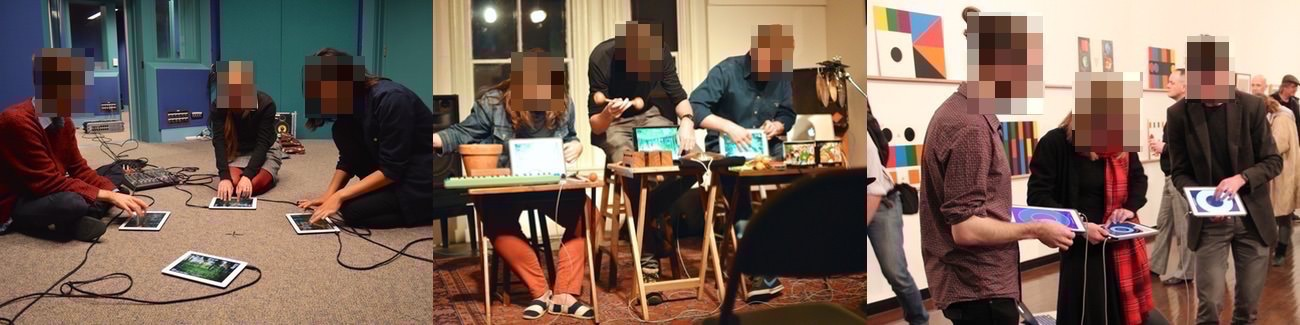
\includegraphics[width=\linewidth]{figures/three-performance-contexts}
  \caption{Collaborative musical interaction with our touch-screen
    interfaces in three different contexts: (left to right) rehearsal
    in a studio,
    performance in front of an audience, and demonstration at a
    research poster session. All of these session were improvised,
    and in the performance session, the musicians used percussion
    instruments as well as iPads.
    \label{fig:three-performance-contexts}}
\end{figure*}


Finally, we report a quantitative analysis of the transition matrices
from our experimental protocols, and describe the quantities
\emph{flux} and \emph{entropy} which can be used to characterise the
gestural activity of the musicians during a performance. We found a
significant effect of the app on these measures, allowing us to
observe quantitatively the performers' dissatisfaction with a
particular interface. We also investigate the significant relationship
between both of these measures and the survey responses, which
suggests that performers rate interaction with our agent and apps more
highly when engaged in adventurous, exploratory performance.

\section{Related Work}

\begin{itemize}
\item Using Markov chains and transition matrices for usability
  modelling~\cite{Thimbleby:2001kq,Thimbleby:2004fj}
\item coding livecoding~\cite{Swift:2014tya}
\end{itemize}

\section{Transition Matrices and Matrix Measures}

It has been recognised that collaborative interactions such as
improvised musical performances can be modelled as a sequence of
states. In the following section we present a method for analysing the
transitions between adjacent states in such a sequence and derive two
high-level quantities that we use to compare musical performances
under different circumstances. Suppose that an collaborative
interaction can be characterised by a set of interaction states $S$
with $m$ members. Each participant's activity can then be represented
as a sequence:
\begin{equation}
 X_n \hskip 2em n = 1, \ldots, N
\end{equation}
Where each $X_i$ is a member of $G$. The transitions between different
interaction states can be summarised in a transition matrix as if the
sequence $X_n$ were a first-order Markov chain. Let $N_{ij}$ be the
number of times that state $j$ follows state $i$. Each participant's
transition matrix, $P$, will then be an $m \times m$ matrix with
entries calculated thus
\begin{equation}
  p_{ij} = \frac{N_{ij}}{\sum_j N_{ij}}
\end{equation}
Each entry of $P$ will be such that the transition probability from
state $i$ to state $j$ is given by the entry in the $i^{th}$ row and
the $j^{th}$ column. The transition activity of the whole ensemble can
be calculated by averaging the transition matrix for each performer.

To compare the transition matrices of different interactions we use
two high-level quantities, ``flux'' and ``entropy''. The flux of a
sequence is defined as the ratio of changed transitions (e.g. state $x$
to state $y$), to self transitions (e.g. state $x$ to state $x$). The
the flux of a transition matrix $P$ can be calculated as:
\begin{equation}
  \mathrm{flux}(P) = 1 - tr(P)
\end{equation}
Where the trace of P, $tr(P)$ is given by the vector 1-norm of the
diagonal entries of $P$. 
% Where $\|P\|_1 = \sum_{i,j}|p_{ij}|$ is the element-wise 1-norm of $P$
% and $\mathrm{diag}(P)$ is the vector of the main diagonal entries of
% $P$.
Intuitively, flux is a measure of how frequently a group changes state. Flux
returns a value in the interval $[0,1]$ and will return 0 when
participants never change state, and 1 when participants never stay on
the same state for two measurements in a row.

A related (but different) high-level derived quantity for the
transition matrix is its entropy, defined in the
information-theoretic~\cite{Shannon:1948rt} sense:
\begin{equation}
  H(P) = -\sum_{i,j}p_{ij}\log_2(p_{ij})
\end{equation}
This entropy measure is small when the matrix is sparse, and largest
when each matrix element is equal. It offers a different perspective
on collaborative interactions than the flux measure by capturing the
breadth of the gestural space explored by the participants throughout
the course of an interaction. Consider the degenerate case of a
participant who alternates between two states for a whole performance:
the flux in this case will be maximal ($\mathrm{flux}(P) = 1$) since
there are no self-transitions, (only $A \rightarrow B$ or
$ B \rightarrow A$) even though the participant has only used a small
subset of the state space. The entropy of this interaction,
on the other hand, will be low. Entropy, therefore, is a measure of
how broad the participant's exploration of the state space is in a given
interaction.

\section{A Corpus of Touch-Screen Interactions}

\begin{table}
%\centering
\begin{tabular}{l|llll}
\hline
            & Total & Min  & Median   & Max     \\ 
\hline
N           & 150       &         &        &  \\
Record size & 306MB     &         &        &   \\
Length      & 20H34M22S & 1M0S    & 7M29S  & 26M0S\\
Participants& 524       & 1       & 4      & 9    \\
Flux        &           & 0.02239 & 0.1445 & 0.3246\\
\hline
\end{tabular}
\caption{
  Representative data about the corpus of musical touch-screen
  interaction sessions used in this study. These sessions were
  rehearsals, performances, studies, and demonstration sessions and the
  participants improvised or performed written compositions. Each record
  consisted of touch-data recorded in CSV format and was later analysed
  with a gestural classification system. Some participants were
  present in multiple sessions, however this data was not tracked in
  the corpus.\label{corpus-table}}
\end{table}


\begin{figure}
  \centering
  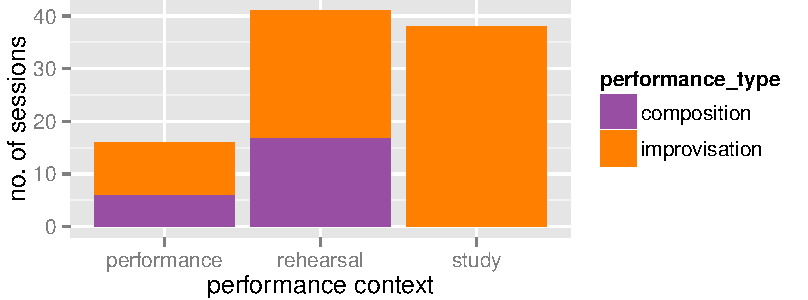
\includegraphics[width=\linewidth]{figures/sessions-count}
  \caption{Distribution of the sessions in our interaction corpus by
    performance context. Improvisations or compositions were repeated
    several times in rehearsals and study sessions but only performed
    once in concerts.
    \label{fig:count-data}}
\end{figure}


In the following sections, we will use transition matrices and the
flux measure to analyse a corpus of data collected as part of our research
into collaborative interactions with musical touch-screen tablet
interfaces. 

Over a period of more than two years (April 2013 - June 2015), we have
collected data from $150$ sessions where various participants used
musical touch-screen interfaces on Apple iPad devices. These
interfaces all shared a common mode of interaction where the majority
of the screen could be used for free form touch interactions; tapping
produced short sounds, while swiping or swirling produced long sounds
with volume proportional to the velocity of the moving touch point.
All touch interactions from each participant in a session was recorded
by sending data to a central server application. This data was stored
in CSV files recording the date and time, X, and Y locations,
velocity, and a unique device identifier for each touch event detected
by the iOS operating system.

Each session took place in a number of contexts including rehearsals,
performances, lab study sessions, classes, and casual demonstrations,
some of which are shown in Figure
\ref{fig:three-performance-contexts}. Participants performed free
improvisations as well as written compositions and performed on iPads
alone or using setups of iPads and acoustic percussion instruments.
The median length of these sessions was 7m29s and the median number of
participants was four, other descriptive statistics about the sessions
is shown in Table \ref{corpus-table}. Each session was coded with
metadata regarding the session context (whether it was a performance,
rehearsal, study, demonstration, or data collection session), the
session type (either improvisation or composition), and the
instruments used (iPads alone, or iPads with acoustic percussion). The
distribution of recorded sessions by context and type is shown in
Figure \ref{fig:count-data}.

To analyse the gestural interactions present in each of these
sessions, the sessions were automatically coded according to a
vocabulary of nine simple, continuous, touch-screen gestures. Examples
of these gestures was generated by an expert user in formal process
where each gesture was performed for 1-minute and feature vectors of
discriptive statistics on these examples was used to train a Random
Forest~\cite{Breiman:2001kx} classifier\footnote{The classifier used
  was from Python's Scikit-learn package~\cite{scikit-learn}.}. The
classifier was applied to 5-second windows of the touch-data each
second provide a chain of gesture-states for each participant in each
session. These chains can be used to create $9 /times 9$
gesture-transition matrices for individual performers, and the whole
ensemble in each session.

While the interaction sessions recorded in our corpus were performed
by many different participants with varying experience levels, in
different contexts and on different instrumental setups, the common
interface and method of recording the data allows all the sessions to
be transformed into gesture sequences. This common format allows us to
ask if performance styles vary in between these different situations.
The sequences can be plotted and inspected qualitatively, but
transition matrices present a quantitative approach to analysing such
interactions.

In the rest of this paper we will use our matrix measure techniques to
interrogate this dataset and to answer two questions. First, do the
transition matrix measures allow us to distinguish between different
performance contexts, types and instrumental setups? Secondly, do
these performance measure allow us further insight into the corpus
than the metadata can provide?

\subsection{Differentiating interaction sessions}
\label{differentiating-interaction-sessions}

\begin{figure}
  \centering
  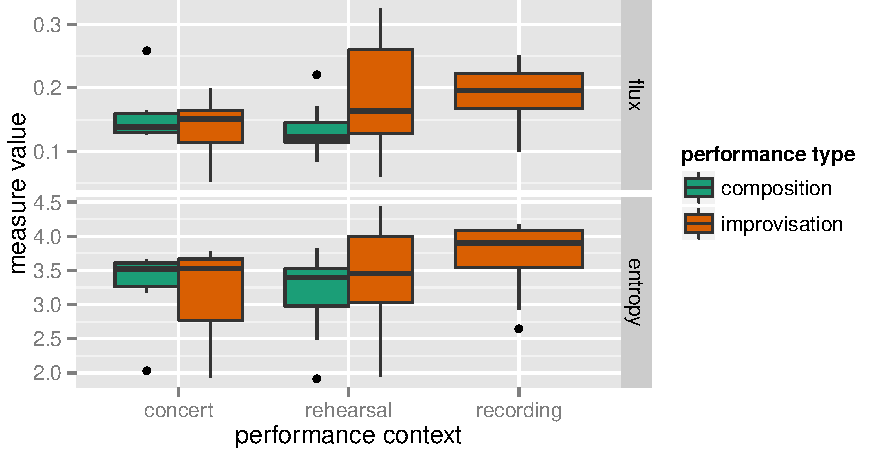
\includegraphics[width=\linewidth]{figures/context-flux-entropy-boxplot}
  \caption{Distributions of flux and entropy values by performance context. Study
    and rehearsal sessions had the highest flux for improvisations
    which fell during performances. Compositions had lower flux in
    rehearsals than performances. Demonstration sessions had much lower entropy
  indicating data unevenly spread in the transition matrices. This
  could be because untrained
  participants did not explore the full gestural potential of the
  instruments. 
  \label{fig:flux-entropy-boxplot}}
\end{figure}

\begin{figure}
  \centering
  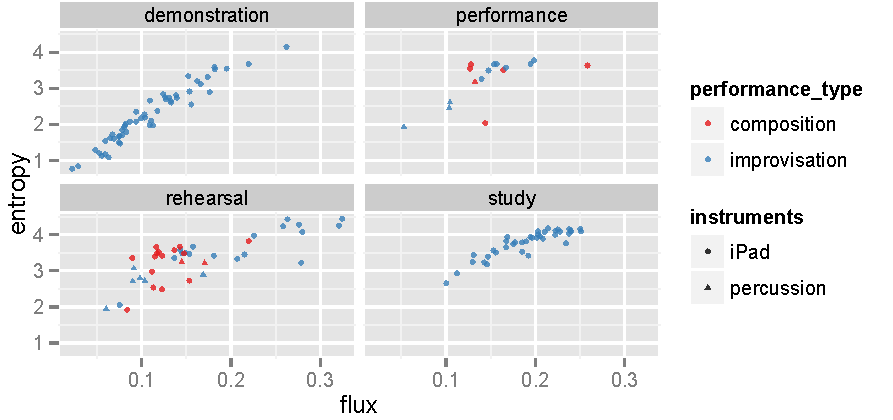
\includegraphics[width=\linewidth]{figures/flux-entropy-distribution}
  \caption{Distribution of flux and entropy by performance type and
    context. Flux and entropy tended to be linearly related in
    improvisations, particularly in demonstrations and studies, while
    compositions had a more scattered relationship.
    \label{fig:flux-entropy-distribution}}
\end{figure}

The distribution of flux and entropy with respect to session contexts,
types and instrumentation are shown in Figures
\ref{fig:flux-entropy-boxplot} and
\ref{fig:flux-entropy-distribution}. A three-way ANOVA procedure was
performed on the data set to find whether the metatdata could
significantly predict the entropy and flux values. In the following
analysis, only the 95 performative sessions were considered (i.e. not
the demonstration or data collection contexts).

All main effects on flux were found to be significant: performance
context ($F(2,86) = 6.28, p < 0.01$), performance type ($F(1,86) =
7.21, p < 0.01$), and instrumentation ($F(1,86) = 20.06, p < 0.001$).
Significant interaction effects were also found for performance
context and type ($F(1,86) = 6.18, p < 0.05$), and performance context and
instrumentation ($F(1,86) = 10.48, p < 0.01$).

For entropy, significant main effects were found due to performance
context ($F(2,86) = 12.10, p < 0.001$), and instrumentation ($F(1,86)
= 25.86$). The interaction of performance type and instrumentation was
also found to be significant ($F(1,86) = 9.93, p<0.01$).

These tests show that the different interaction styles that might be
present in performance contexts, types and
instrumentations are reflected in the values of flux and entropy of
their transition matrices.

% todo need to add overall contrasts column to do pairwise t-tests.

\subsection{Breaking performances into sections}

It is clear that flux and entropy can detect the variation in
performance styles in between performances of different types, but can
they be used to understand some of the internal structure of
performances? A simple model for understanding temporal art-forms is
the ``beginning, middle, end'' structure. To investigate how the
structure fits session in our corpus, we can divide the
gestural-sequences of each session into thirds and calculate the
transition matrices given by each section.

Figures \ref{fig:type-section-flux-entropy} shows that the flux and
entropy of compositions are much more stable with respect to section
than for improvisations. The stability of compositions is to be
expected since performers are expected to use the same gestures in
each rehearsal and performance of a composition, it may be that
different kinds of compositions could result in different structural
differences. Both measures have a downward trend through sections in
improvisations with Kruskal-Wallis tests showing a significant effect
of section on flux ($\chi^2(2)=5.8, p=0.05$). This could be explained
by performers entering an exploration stage at the start of an
improvisation, where they change gesture frequently to experiment with
different ideas. At the end of an improvisation, performers may change
gesture less frequently while ``winding up'' the performance.

The gestural change in improvisation can be further explored by
dividing the sessions by performance context. Figure
\ref{fig:context-section-flux-entropy} shows this division for
improvisations only. In rehearsals and studies the distribution of
flux and entropy over sections has a similar shape, both measures drop
in the ending section of studies and after the beginning section in
rehearsals. In performances however, flux drops after the beginning
while entropy drops substantially in the ending section. This
indicates a more constrained performance style in this closing
section, where performers transition between fewer gestures in the
final section of performances.

% todo add the plots here.

\begin{figure}
  \centering
  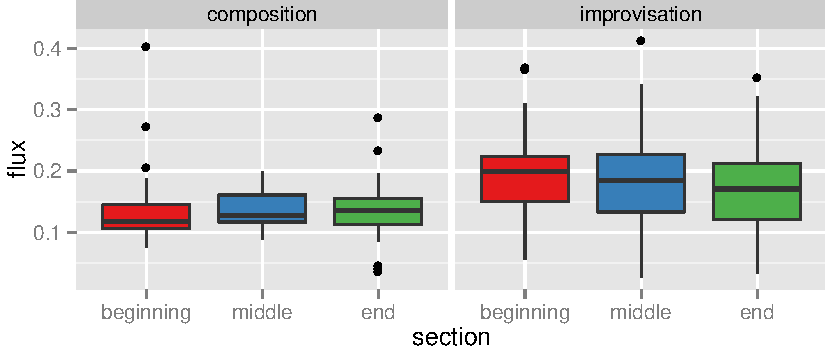
\includegraphics[width=\linewidth]{figures/type-section-flux}
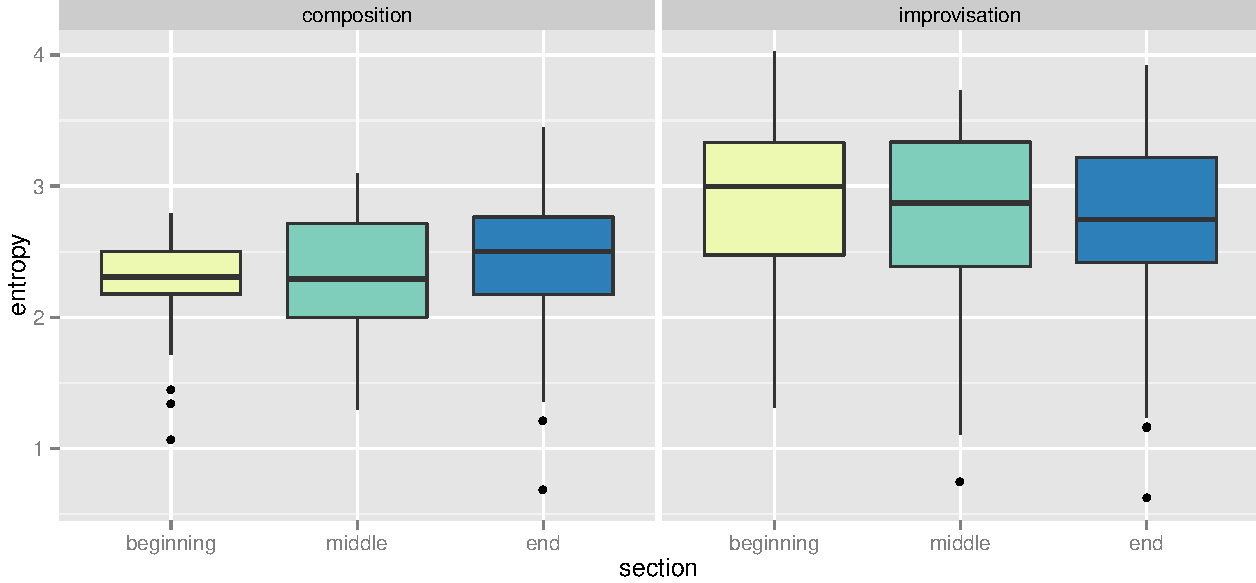
\includegraphics[width=\linewidth]{figures/type-section-entropy}
  \caption{The flux of compositions and improvisations divided into
    beginning, middle, and end. Composition flux remains stable throughout,
    but improvisations show a downward trend and composition entropy tends to move up
    at the end, while flux moves down.
    \label{fig:type-section-flux-entropy}}
\end{figure}

\begin{figure}
  \centering
  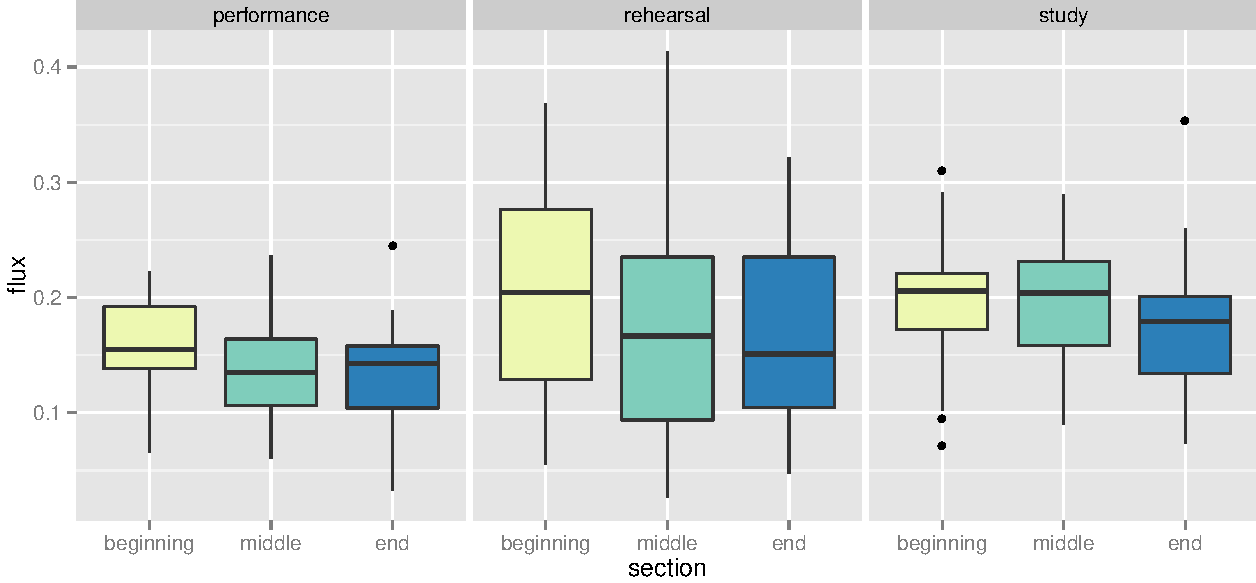
\includegraphics[width=\linewidth]{figures/context-section-flux}
  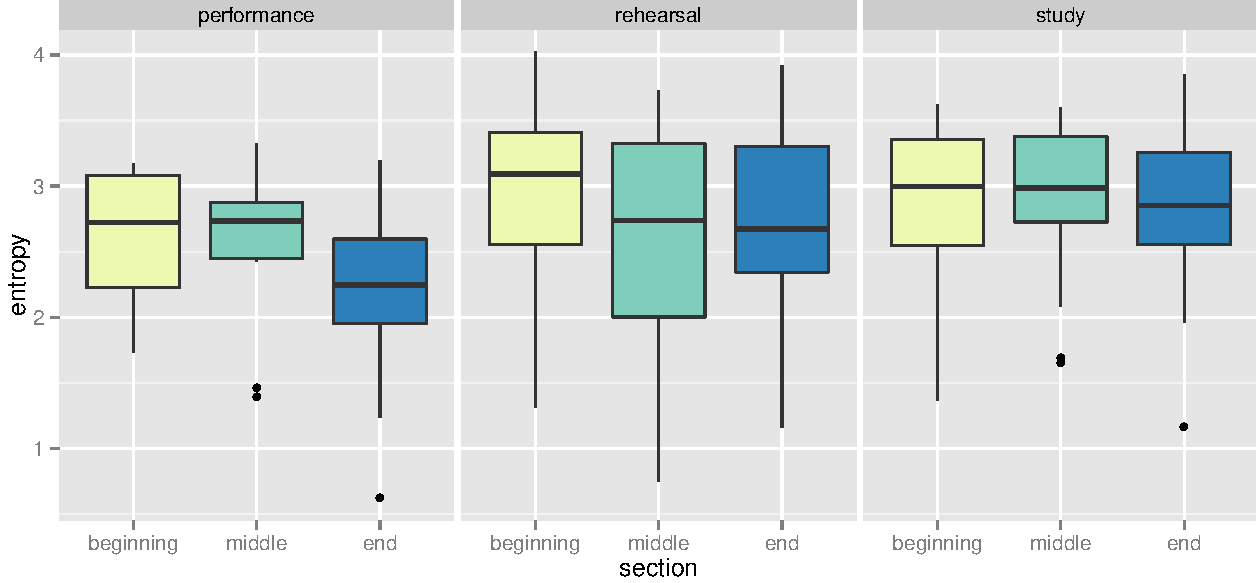
\includegraphics[width=\linewidth]{figures/context-section-entropy}
  \caption{The distribution of flux and entropy in performances divided by ``beginnings,
    middles, and ends''.
    \label{fig:context-section-flux-entropy}}
\end{figure}



\subsection{Performance styles over time}

While the interaction session in our corpus have many different
contexts, they are all part of a program of artistic and HCI research
that has evolved over time. Figure \ref{fig:flux-entropy-through-time}
shows the values of flux and entropy for each session in the corpus.
Over the course of this research program, different ensembles and
different activities have been emphasised, some of these differences
can be seen as clusters of performances with similar flux and entropy
in the two plots. For instance, the earliest series of rehearsals and
performances had flux between 0.05 and 0.15, while the period of
activity after July 2014 had flux between 0.1 and 0.25. This change
corresponded with an intensive series of study sessions and rehearsals
where the participants developed a more fluctuating style of
performance. The entropy between these two periods, however, remains
at a similiar level, showing the the space of available gestures that
the performers explored was more constant.

\begin{figure}
  \centering
  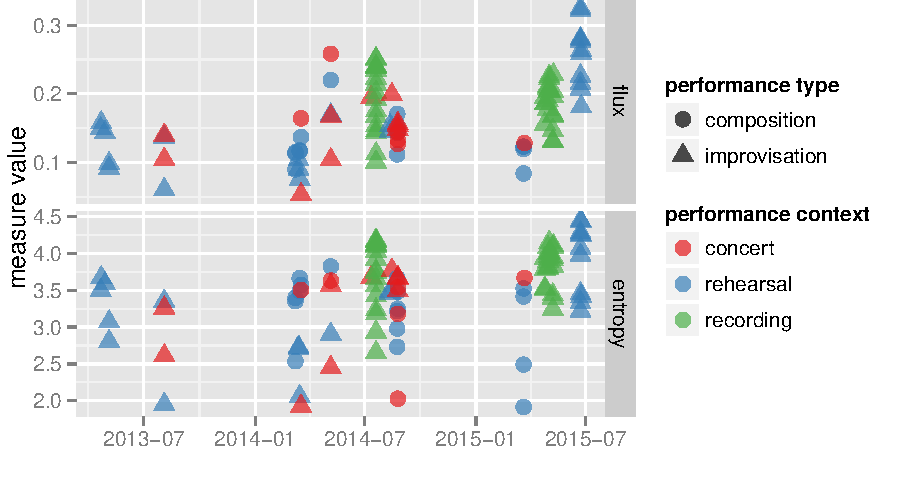
\includegraphics[width=\linewidth]{figures/flux-entropy-through-time}
  \caption{Distribution of flux and entropy values of sessions through time.
    Different performance styles are visible as clusters of similar
    flux regardless of performance context.
    \label{fig:flux-entropy-through-time}}
\end{figure}

\section{Conclusions}

In this paper we have extended the transition matrix methodology
previously presented at CHI with two simple matrix measures, flux and
entropy, both of which have been demonstrated to have significant
discriminatory power with regards to a corpus of 150 collaborative
touch-screen interactions. Not only do these measures differentiate
between different types of sessions and the internal structure of
these sessions, but they have explanatory power that has thrown new
light on the musical interactions under examination. HCI researchers
are increasingly concerned with interactions that happen in-the-wild,
where the interactions of many users may be collected without the
opportunity to survey or interview users. We suggest that analysing
interaction-state transitions using matrices and simple measures can
lead to new insights into HCI interactions outside the lab.

% todo blah de blah

% \section{Modelling Performer Ratings with Flux and Entropy}

% \begin{figure}
%   \centering
%   \includegraphics[width=\linewidth]{figures/stat-response-fit.pdf}
%   \caption{Transition matrix statistics (flux above and entropy below) vs Likert responses for
%     questions 3, 6 and 7, all of which exhibited significant
%     relationships under a proportional odds logistic regression model.
%     A least-squares linear model is shown with a dotted line.
%     \label{fig:stat-response-fit}}
% \end{figure}

% One final question to explore is how these flux and entropy measures
% in the interaction data relate to the performers' perceptions of their
% performance?

% To answer this question, we construct models with the flux and entropy
% measures as independent variables and the Likert responses (1 to 5) as
% the dependent variable. These measures exhibited clear relationships
% for three of the survey questions (Questions 3, 6 and 7), which are
% plotted in Figure~\ref{fig:stat-response-fit} where the least-squares
% line of best fit has a positive gradient for both flux and entropy.

% Determining the strengths of these positive relationships is
% difficult, both due to the problem of treating ordinal Likert
% responses as numeric~\cite{Gardner:2007fj} and also
% due to the unknown distribution of the entropy and flux statistics. As
% a result, we use a conservative proportional odds logistic regression
% (POLR)~(using the \texttt{polr} function in \texttt{R}, from the MASS
% package \cite{Venables:2002qv}) to treat the Likert responses as an
% ordered factor response.

% The POLR results indicate a significant ($p<0.05$) relationship
% between the user-reported Likert response and the flux statistic for
% Question 3 ($t = 2.77, df = 4, p = 0.025$), Question 6
% ($t = 2.41, df = 4, p = 0.037$), and Question 7
% ($t = 2.49, df = 4, p = 0.034$). The same questions displayed a
% significant relationship for the entropy statistic: Question 3
% ($t = 2.93, df = 4, p = 0.022$), Question 6
% ($t = 2.69, df = 4, p = 0.028$), and Question 7
% ($t = 2.89, df = 4, p = 0.022$). These relationships are shown in
% Figure~\ref{fig:stat-response-fit}.

% It is notable that these questions (3, 6, and 7) all pertain to the
% \emph{perceived effect of the agent} on the performers. As the agent
% uses the flux measure to trigger new-idea messages, it appears that
% performers appreciated its intervention more in particularly creative
% performances where flux and entropy were high.






\bibliographystyle{SIGCHI-Reference-Format}
\bibliography{references}

\end{document}

%%% Local Variables:
%%% mode: latex
%%% TeX-master: t
%%% End:
